\documentclass[10pt,c,aspectratio=1610,handout]{beamer}
\usetheme[block=fill,numbering=fraction,progressbar=frametitle]{metropolis}
%\usecolortheme{beaver}
\usepackage{textpos}
\usepackage{amsmath}
\usepackage{amssymb}
\usepackage{appendixnumberbeamer}

\setbeamercovered{transparent}

\newcommand\blfootnote[1]{%
  \begingroup
  \renewcommand\thefootnote{}\footnote{#1}%
  \addtocounter{footnote}{-1}%
  \endgroup
}

\renewcommand{\baselinestretch}{1.25}
% Colour theme
\definecolor{QDMblue}{rgb}{0.00, 0.1882, 0.3608}
\definecolor{QDMgold}{rgb}{0.9098, 0.6510, 0.0000}
\definecolor{QDMgreen}{rgb}{0.3098, 0.5490, 0.0510}
\setbeamercolor{normal text}{ fg= QDMblue , bg= white }
\setbeamercolor{alerted text}{ fg= QDMgold }
\setbeamercolor{example text}{ fg= QDMgreen }

\begin{document}

% Personal Info
\title{Lecture 04: Monetary Policy, Price-Setting,\\and Information Frictions}%
\author[Konstantin Gantert]{\begin{large} Konstantin Gantert \end{large} \\ \textbf{Quantitative Dynamic Macroeconomics}}
\date{\textit{this version:} \today}

% Eliminates Navigation Bar on every Frame
\beamertemplatenavigationsymbolsempty

%-------------------------------------------------------------------------
% 0.1 Titlepage
%-------------------------------------------------------------------------
{\setbeamertemplate{footline}{} 
\frame{\titlepage}}
 \addtocounter{framenumber}{-1}
%-------------------------------------------------------------------------
% Outline for this Lecture
\begin{frame}{Outline for this Lecture}%
  \onslide<1->{%
  \begin{minipage}{0.48\textwidth}%
    \textbf{What have we seen so far}%
    \begin{enumerate}%
      \item Stochastic CiA Model {\tiny [CG 1, 2, 3, 5]}%
      \item Markov Process Computer Model {\tiny [CG 3, 4]}%
      \item AR(1) Process Computer Model {\tiny [CG 3, 4]}%
      \item Calculating Model Statistics {\tiny [CG 2, 3, 4]}%
    \end{enumerate}%
  \end{minipage}}%
  \hfill%
  \onslide<3->{%
  \begin{minipage}{0.48\textwidth}%
    \textbf{What we will see today}%
    \begin{enumerate}%
      \item Monetary policy rules {\tiny [CG 6]}%
      \item Monopolistic competition {\tiny [CG 1, 3, 5]}%
      \item Information frictions {\tiny [CG 1, 5]}%
      \item Impulse response functions {\tiny [CG 3, 4]}%
    \end{enumerate}%
  \end{minipage}}%
  \vspace*{0.25in}%
  \onslide<2->{%
  \begin{block}{Big Picture of the Lecture:}%
    \begin{enumerate}%
      \item How to set monetary policy goals, targets, and instruments?%
      \item How do households set their goods prices under market power?%
      \item What role does uncertainty within period money growth play for aggregate demand?%
    \end{enumerate}%
  \end{block}}%
\end{frame}%
%-------------------------------------------------------------------------
% BLOCK 1: Money Supply Rules and Interest Rate Rules
%-------------------------------------------------------------------------
\section{Money Supply Rules and\\Interest Rate Rules\\{\small Cole (2020) chapter 9}}%
%-------------------------------------------------------------------------
% US Central Bank Policy through Time
\begin{frame}{US Central Bank Policy through Time}%
  We can order US central bank policy by the Federal Reserve in roughly five episodes since the second world war:%
  \begin{itemize}%
    \item[$\blacktriangleright$] \textbf{Mid 1960s to 1979:} Inflation targeting regime with aim to create high inflation for driving down unemployment (and finance Vietnam war).%
    \item[$\blacktriangleright$] \textbf{Oct 1979 to Oct 1982:} Price level targeting in a regime of monetary tightening as inflation (expectations) were high alongside high unemployment.%
    \item[$\blacktriangleright$] \textbf{Oct 1982 to 2008:} Interest rate targeting with explicit price stability and employment targets (Great Moderation).%
    \item[$\blacktriangleright$] \textbf{2009 to 2015:} Zero interest rate policy (and quantitative easing) following the Great Recession (financial crisis that started end of 2006).%
  \end{itemize}%
  \pause%
  \vspace{0.1in}%
  \begin{center}%
    How is monetary policy in the US (the EMU) conducted since then?%
  \end{center}%
\end{frame}%
%-------------------------------------------------------------------------
% Augmented Model
\begin{frame}{Augmented Model}%
  We augment our stochastic CiA model to include a policy margin through \textbf{preference shocks}!\vspace{0.1in}\\%
  \pause%
  \textbf{Modified flows of utility:}%
  \begin{align}%
    u(C_t) - \left( 1 + \Upsilon_t \right) v(L_t)%
  \end{align}%
  \vspace{-0.2in}%
  \begin{itemize}%
    \small%
    \item[$\blacktriangleright$] $\Upsilon_t$ is a shock to the \textbf{disutility of labor} making households more or less willing to work.%
  \end{itemize}%
  \pause%
  The \textbf{only FOC that changes} is the labor FOC given by:%
  \begin{align}%
    \left(1+\Upsilon_t\right) v^{\prime}(L(s^t)) L(s^t) \; = \; \frac{\beta}{1+\tau_t(s^t)}%
  \end{align}%
  \vspace{-0.2in}%
  \begin{itemize}%
    \small%
    \item[$\blacktriangleright$] AR(1)-process: $\Upsilon_t = \rho_\Upsilon \Upsilon_{t-1} + \sigma_\Upsilon \upsilon_t$%
    \item[$\blacktriangleright$] The implied level of labor supply is efficient.%
  \end{itemize}%
  \pause%
  \vspace{0.1in}%
  However, we assume that the central bank wants to stabilize the economy at its original level.%
  \begin{align}%
    v^{\prime} (\bar{L}) \bar{L} \; = \; \frac{\beta}{1+\bar{\tau}}%
  \end{align}%
  \vspace{-0.2in}%
\end{frame}%
%-------------------------------------------------------------------------
% Money Supply Rules
\begin{frame}{Money Supply Rules}%
  Central bank \textbf{sets their money supply} given  expectations about $\tilde{\Upsilon}_t$ to achieve its target $\bar{L}$:%
  \begin{align}%
    \left( 1+ \tilde{\Upsilon}_t\right) v^{\prime}\left(\bar{L}\right) \bar{L} \; = \; \frac{\beta}{1+\tau\left(\tilde{\Upsilon}_t\right)}
  \end{align}%
  where $\tilde{\Upsilon}_t = \mathbb{E}_t \Upsilon_t$ {\small(shocks this period are unexpected)}. Monetary policy ...%
  \pause%
  \begin{itemize}%
    \item[$\blacktriangleright$] smoothes out changes in $\Upsilon_t$ to the extend that they are expected.%
    \item[$\blacktriangleright$] is backward-looking as the shock process and its implications for the economy depend on the persistence parameter of the AR(1) process.%
  \end{itemize}%
  \vspace{0.1in}%
  \pause%
  \begin{center}%
    What if there is a persistent shift in $\Upsilon_t$ that the central bank does not see?%
  \end{center}%
\end{frame}%
%-------------------------------------------------------------------------
% Inflation Targeting
\begin{frame}{Inflation Targeting}%
  A central bank targets some level of the inflation rate which is given in the model by%
  \begin{align}%
    1+\pi_t \; = \; \frac{P_{t+1}}{P_t} \; = \; \frac{M_{t+1} C_{t}}{M_t C_{t+1}} \; = \; \frac{\left(1+\tau_t\right) L\left(\Upsilon_t, \tau_t\right)}{\left(1+g_{t+1}\right) L\left(\Upsilon_{t+1}, \tau_{t+1}\right)}
  \end{align}%
  \pause%
  In order for the central bank to be able to implement this policy rule, it needs to ...%
  \begin{itemize}%
    \item[$\blacktriangleright$] forecast the future growth rate, $g_{t+1}$.%
    \item[$\blacktriangleright$] forecast the future labor supply disutility, $\Upsilon_{t+1}$.%
    \item[$\blacktriangleright$] commit to its own future money growth rate, $\tau_{t+1}$.%
  \end{itemize}%
  \vspace{0.1in}%
  \pause%
  \begin{center}%
    Can a central bank accurately and persistently forecast the future?\\%
    Do households and firms belief the central bank is comitted to its future interest rates?%
  \end{center}%
\end{frame}%
%-------------------------------------------------------------------------
% Interest Rate Rules
\begin{frame}{Interest Rate Rules}%
  A central bank sets the penalty price of the budget constraint by setting the interest rate:%
  \begin{align}%
    \mu(s^t) \; = & \; \frac{\sum_{s^{t+1} \in S^{t+1}(s^t)} \mu(s^{t+1})}{q_t}\notag\\%
    \pause%
    \Leftrightarrow \quad \quad \mu_t \; = & \; \mathbb{E}_t \frac{\mu_{t+2}}{q_t \cdot q_{t+1}} \; = \; \mathbb{E}_t \frac{\mu_{t+T+1}}{\prod_{i=0}^T q_{t+i}}%
  \end{align}%
  \pause%
  \textbf{Implications:}%
  \begin{itemize}%
    \item[$\blacktriangleright$] Future interest rates, $q_{t+1}$, impact $\mu_t$ the same as current interest rates.%
    \item[$\blacktriangleright$] However, future interest rates, $q_{t+1}$, will also affect future $\mu_{t+1}$.%
    \pause%
    \item[$\blacktriangleright$] \textbf{Forward guidance:} The fact that future interest rates affect today's economy encourages central banks even more to forecast the future.%
  \end{itemize}%
  \vspace{0.1in}%
  \pause%
  \begin{center}%
    Does the central bank understand the impact of interest rates on the economy?%
  \end{center}%
\end{frame}%
%-------------------------------------------------------------------------
% Monetary Policy in the CiA Model
\begin{frame}{Monetary Policy in the CiA Model}%
  What are the goals, targets, and instruments used by a central bank?%
  \begin{itemize}%
    \item \textbf{Money supply:} Do we observe unbiased shocks in real-time?%
    \item \textbf{Inflation targeting:} Do we observe unbiased shocks in real-time and can forecast the future accurately?%
    \item \textbf{Interest rate:} Do we understand the link between interest rates and targets variables (inflation or employment stability) in our ecomnomy correctly?%
  \end{itemize}%
  \pause%
  \begin{block}{Taylor Rule}%
    \small%
    John B. Taylor described and estimated a rule for US monetary policy in a series of papers. The rule named after him describes consistently how the FED behaves:%
    \begin{align}%
      \normalsize%
      i_t \; = \; \pi_t + r_t^* + 0.5\left(\pi_t-\pi_t^*\right) + 0.5\left(y_t - \bar{y}_t\right)%
    \end{align}%
  \end{block}%
\end{frame}%
%-------------------------------------------------------------------------
% BLOCK 1: The Demand Function of Differentiated Goods
%-------------------------------------------------------------------------
\section{The Demand Function of Differentiated Goods\\{\small Cole (2020) chapter 10.1}}%
%-------------------------------------------------------------------------
% Money and the Business Cycle
\begin{frame}{Money and the Business Cycle}%
  \begin{itemize}%
    \item[$\blacktriangleright$] Many people believe that increases in money ...%
    \begin{itemize}%
      \item[$\rightarrow$] ... increases nominal demand,%
      \item[$\rightarrow$] ... and this in turn increases output and employment.%
    \end{itemize}%
    \vspace*{0.2in}%
    \pause%
    \item[$\blacktriangleright$] This is a bit surprising because ...%
    \begin{itemize}%
      \item[$\rightarrow$] ... if money doubles prices double and nothing really has changed.%
      \item[$\rightarrow$] ... money in the long-run seems neutral for this reason.%
    \end{itemize}%
    \vspace*{0.2in}%
    \pause%
    \item[$\blacktriangleright$] Many argue that some element of ''surprise'' is important here.%
  \end{itemize}%
\end{frame}%
%-------------------------------------------------------------------------
% The Element of Surprise in Money Increases
\begin{frame}{The Element of Surprise in Money Increases}%
  \begin{center}%
    \begin{large}%
      \emph{Do surprise increases in money supply have an impact on the economy?}%
    \end{large}%
  \end{center}%
  \pause%
  \begin{itemize}%
    \item[$\blacktriangleright$] \textbf{Historical evidence:} 
    \begin{itemize}%
      \item[$\rightarrow$] The long-depression in the UK after WWI.%
      \item[$\rightarrow$] The rebound when inflation returned during the Great Depression.%
    \end{itemize}%
    \pause%
    \item[$\blacktriangleright$] \textbf{Evidence from vector-auto-regressions (VARs):}%
    \begin{itemize}%
      \item[$\rightarrow$] This is a standard sort of VAR equation%
      \begin{align*} %
        y_t = A + B y_{t-1} + C ( m_t - E_{t-1} m_t ) + D x_t + \epsilon_t %
      \end{align*}%
      \item[$\rightarrow$] We need assumptions to determine money growth expectations and to estimate their effect.%
      \item[$\rightarrow$] Different approaches, and at least some suggest reasonably sizable and moderately persistent effects.%
    \end{itemize}%
    \pause%
    \item[$\blacktriangleright$] \textbf{Further method:} Directly date ''surprise'' changes in central bank policy and see what happened.%
    \vspace*{0.1in}%
    \pause%
    \item[$\Rightarrow$] This evidence led to the development of New Keynesian models with price-setting frictions. \textbf{We will adjust our model accordingly!}%
  \end{itemize}%
\end{frame}%
%-------------------------------------------------------------------------
% Step 1: Putting Price-Setting in our Model
\begin{frame}{Step 1: Putting Price-Setting in our Model}%
  \textbf{Starting point:} Changing the model setup!%
  \begin{itemize}%
    \item[$\blacktriangleright$] Go back to the original set-up (lecture 1) with multiple goods indexed by $i\in I$.%
    \item[$\blacktriangleright$] Each good is produced by an individual producer, which chooses her price $P(i)$.%
    \item[$\blacktriangleright$] Each producer has to meet any demand once the price is set.%
    \pause%
    \item[$\blacktriangleright$] The \textbf{composite good} is determined by an aggregator of the individual goods:%
    \begin{align*}%
      C \; = \; \left\{ \frac{1}{\#I}\sum_{i\in I}C(i)^{\rho} \right\}^{\frac{1}{\rho}}%
    \end{align*}%
    \begin{itemize}%
      \item[$\rightarrow$] The household's preferences are again given by $u(C)$.%
      \item[$\rightarrow$] Individual production is $C(i)$, labor is $C(i)/Z$, and revenue is $P(i)C(i)$.%
    \end{itemize}%
  \end{itemize}%
\end{frame}%
%-------------------------------------------------------------------------
% Step 2: Deriving the Demand Function (1/5)
\begin{frame}{Step 2: Deriving the Demand Function (1/5)}%
  Derive the optimal composition of individual goods given some fixed money holdings.%
  \pause%
  \begin{itemize}%
    \item[$\blacktriangleright$] Lagrangian of a household's optimal expenditure problem: spending $M$ to maximize $C$:%
    \begin{align*}%
      \mathcal{L} \; = \; \max_{C(i)}\min_{\lambda} \left\{ \frac{1}{\#I}\sum_{i\in I}C(i)^{\rho} \right\}^{\frac{1}{\rho}} + \lambda \left\{ M-\sum_{i}P(i)C(i) \right\}.%
    \end{align*}%
    \pause%
    \item[$\blacktriangleright$] The \textbf{first-order condition} is given by%
    \begin{align*}%
      \frac{\partial \mathcal{L}}{\partial C_t(i)}: & \quad \left\{ \frac{1}{\#I} \sum_{i \in I}C(i)^{\rho} \right\}^{\frac{1}{\rho}-1} \frac{1}{\#I}C(i)^{\rho-1} \; = \; \lambda P(i)\\%
      \implies \quad & \quad C^{1-\rho} \frac{1}{\#I}C(i)^{\rho-1} = \lambda P(i).%
    \end{align*}%
    \pause%
    \item[$\blacktriangleright$] Further note:%
    \begin{align*}%
      \frac{\partial \mathcal{L}}{\partial M} \; = \; \lambda,%
    \end{align*}%
    so $\lambda$ is the value of money in terms of a unit of composite consumption.%
  \end{itemize}%
\end{frame}%
%-------------------------------------------------------------------------
% Step 2: Deriving the Demand Function (2/5)
\begin{frame}{Step 2: Deriving the Demand Function (2/5)}%
  A \textbf{price index} is a way of saying what something costs:%
  \pause%
  \begin{itemize}%
    \item[$\blacktriangleright$] A price index $\bar P$ for composite consumption says that $C$ units cost $\bar P \times C$ units of money.%
    \pause%
    \item[$\blacktriangleright$] While $\lambda$ says $1$ unit of money will get me $\lambda$ units of $C$, so $\bar P = \lambda^{-1}$.%
    \pause%
    \item[$\Rightarrow$] Inserting the price index $\bar{P}^{-1}$ for $\lambda $ in our FOC, we get that%
    \begin{align}%
      \frac{1}{\#I}C(i)^{\rho -1} \; = \; \frac{P(i)}{\bar{P}}C^{\rho -1}.\label{eq:demand_function_1}%
    \end{align}%
  \end{itemize}%
\end{frame}%
%-------------------------------------------------------------------------
% Step 2: Deriving the Demand Function (3/5)
\begin{frame}{Step 2: Deriving the Demand Function (3/5)}\label{slide:demand_function}%
  \begin{itemize}%
    \item[$\blacktriangleright$] Rearranging (\ref{eq:demand_function_1}), we get a nice form for the \textbf{demand function}:%
    \begin{align}%
      \begin{split}\label{eq:demand_function_2}%
        C(i) \; & = \; \left[ \#I\frac{P(i)}{\bar{P}}\right]^{\frac{1}{\rho-1}} C \\%
      & = \; D\left( \frac{P(i)}{\bar{P}}\right)%
      \end{split}%
    \end{align}%
    \pause%
    \item[$\blacktriangleright$] From (\ref{eq:demand_function_2}) we can derive the \textbf{slope of the demand function}:%
    \begin{align*}%
      \frac{d D\left( \frac{P(i)}{\bar{P}}\right)}{dP(i)} \; = \; D\left( \frac{P(i)}{\bar{P}}\right) \times \frac{1}{\rho -1}P(i)^{-1}%
    \end{align*}%
    \pause%
    \item[$\blacktriangleright$] The \textbf{elasticity} is then given by:%
    \begin{align*}%
      \frac{1}{\rho -1}%
    \end{align*}%
  \end{itemize}%
\end{frame}%
%-------------------------------------------------------------------------
% Step 2: Deriving the Demand Function (4/5)
\begin{frame}{Step 2: Deriving the Demand Function (4/5)}%
  But what exactly is our price index $\bar P$?%
  \pause%
  \begin{itemize}%
    \item[$\blacktriangleright$] For everything to add up:%
    \begin{align}%
      M \; & = \; \bar{P} C \; = \; \sum_{i \in I} P(i) C(i) \; = \; \sum_{i \in I} P(i) \left[\# I \lambda P(i) \right]^{\frac{1}{\rho-1}} C \notag\\%
      \pause%
      & \implies \bar P  = \sum_{i \in I} P(i) \left[\# I \frac{P(i)}{\bar P} \right]^{\frac{1}{\rho-1}} \notag\\%
      \pause%
      & \implies \bar{P}=\left\{ (\#I)^{\frac{1}{\rho-1}}\sum_{i}P(i)^{\frac{\rho }{\rho -1}}\right\}^{\frac{\rho -1}{\rho }}%
    \end{align}%
  \end{itemize}%
\end{frame}%
%-------------------------------------------------------------------------
% Step 2: Deriving the Demand Function (5/5)
\begin{frame}{Step 2: Deriving the Demand Function (5/5)}%
  There's a units problem here since \[ C = \left\{ \frac{1}{\#I}\sum_{i\in I} C(i)^{\rho} \right\}^{\frac{1}{\rho}} \] implies that one unit of each good $i$ leads to one unit of the composite good.%
  \vspace*{0.15in}%
  \pause%
  \begin{itemize}%
    \item[$\blacktriangleright$] So in total it takes $\#I$ units of the different goods to get the composite.%
    \pause%
    \item[$\blacktriangleright$] Hence, when all prices are symmetric, $P(i) = P$, it follows $\bar P = \#I \times P$.%
    \pause%
    \item[$\blacktriangleright$] This is something we saw before and just need to adjust $Z$ \[ PZ = \bar P Z / \#I. \]%
    \pause%
    \item[$\blacktriangleright$] We ignore this small distinction going forward because it won't matter for anything.%
  \end{itemize}%
\end{frame}%
%-------------------------------------------------------------------------
% BLOCK 2: Optimal Price Setting
%-------------------------------------------------------------------------
\section{Optimal Price Setting\\{\small Cole (2020) chapter 10.1}}%
%-------------------------------------------------------------------------
% Step 3: The Household's 2-Period Problem (1/4)
\begin{frame}{Step 3: The Household's 2-Period Problem (1/4)}%
  \begin{align*}%
    \max_{\left\{ C_{t},P_{t}(i),M_{t+1},B_{t+1}\right\}_{t=1,2}} & \quad u(C_{1})-v\left( D\left( \frac{P_{1}(i)}{\bar{P}_{1}}\right) / Z_{1}\right)\\%
    & \quad +\beta \left[ u(C_{2})-v\left( D\left( \frac{P_{2}(i)}{\bar{P}_{2}}\right) /Z_{2}\right) \right] +\beta ^{2}V(M_{3},B_{3})%
  \end{align*}%
  subject to%
  \begin{align*}%
    M_{t} \; & \geq \; \bar{P}_{t} C_{t}\\%
    P_{t}(i) D\left( \frac{P_{t}(i)}{\bar{P}_{t}} \right) + \left[ M_{t}-\bar{P}_{t}C_{t}\right] + B_{t}+T_{t} \; & \geq \; M_{t+1} + q_{t}B_{t+1}%
  \end{align*}%
  \pause%
  \begin{itemize}%
    \item[$\rightarrow$] \textbf{Assumption:} We impose the condition that the household must work enough to satisfy demand for its product given the price it sets and the overall price index $\bar{P}$.%
  \end{itemize}%
\end{frame}%
%-------------------------------------------------------------------------
% Step 3: The Household's 2-Period Problem (2/4)
\begin{frame}{Step 3: The Household's 2-Period Problem (2/4)}%
  Three of our FOCs are \textbf{completely unchanged!}%
  \pause%
  \begin{itemize}%
    \item[$\blacktriangleright$] The \textbf{FOC for consumption} is given by:%
    \begin{align*}%
      \beta^{t-1} u^{\prime}(C_t) - \bar{P}_t [ \lambda_t + \mu_t ] \; & \overset{!}{=} \; 0 \\%
      \implies  \frac{\beta^{t-1}} {Z_t L_t} \; & = \; \bar{P}_t [ \lambda_t + \mu_t ] \quad \text{ in equilibrium with log preferences} \\%
      \implies  \beta^{t-1} \; & = \; \bar{M}_t [ \lambda_t + \mu_t ] \quad \text{ because the CiA says } \bar{P}_t C_t = \bar{M}_t = \bar{P}_t Z_t L_t%
    \end{align*}%
    \vspace*{-0.2in}%
    \begin{itemize}%
      \item[$\rightarrow$] $\bar{M}_t$ is whatever amount of money they have in the goods market.%
    \end{itemize}%
    \vspace*{0.1in}%
    \pause%
    \item[$\blacktriangleright$] The \textbf{FOC for money} is given by:%
    \begin{align*}%
      -\mu_t + [ \mu_{t+1} + \lambda_{t+1} ] \; & \overset{!}{=} \; 0 \quad \quad \implies \mu_t \; = \; \frac{\beta^t}{\bar{M}_{t+1}}%
    \end{align*}%
    \pause%
    \item[$\blacktriangleright$] The \textbf{FOC for bonds} is given by:%
    \begin{align*}%
      -q_t \mu_t + \mu_{t+1} \; = \; 0%
    \end{align*}%
  \end{itemize}%
\end{frame}%
%-------------------------------------------------------------------------
% Step 3: The Household's 2-Period Problem (3/4)
\begin{frame}{Step 3: The Household's 2-Period Problem (3/4)}%
  \begin{itemize}%
    \item[$\blacktriangleright$] The \textbf{FOC for pricing} is then given by:%
    \begin{align*}%
      0 \; \overset{!}{=} & \; -\beta^{t-1} v^{\prime} \left( \frac{D \left( \frac{P_{t}(i)}{\bar{P}_{t}}\right)}{Z_t} \right) \frac{1}{Z_{t}} \frac{d}{dP_{t}(i)} D\left( \frac{P_{t}(i)}{\bar{P}_{t}}\right)\\%
      & \; + \mu_{t} \left[ D \left( \frac{P_{t}(i)}{\bar{P}_{t}}\right) + P_{t}(i) \frac{d}{dP_{t}(i)} D \left( \frac{P_{t}(i)}{\bar{P}_{t}}\right) \right]\\%
      \\%
      \pause%
      \Leftrightarrow \quad 0 \; \overset{!}{=} & \; -\beta^{t-1} v^{\prime}\left( \frac{ D \left( \frac{P_{t}(i)}{\bar{P}_{t}}\right)}{Z_t} \right) \frac{1}{Z_{t}} D\left( \frac{P_{t}(i)}{\bar{P}_t} \right) \frac{1}{\rho-1}P_{t}(i)^{-1}\\%
      & \; +\mu_{t} \left[ D \left( \frac{P_{t}(i)}{\bar{P}_{t}} \right) + D \left( \frac{P_{t}(i)}{\bar{P}_t} \right) \frac{1}{\rho-1} \right]\\%
      \\%
      \pause%
      \Leftrightarrow \quad 0 \; \overset{!}{=} & \; -\beta^{t-1} v^{\prime} \left( \frac{D \left( \frac{P_{t}(i)}{\bar{P}_{t}} \right)}{Z_t} \right) \frac{1}{Z_{t}} P_{t}(i)^{-1} + \mu_{t} \rho.%
    \end{align*}%
  \end{itemize}%
\end{frame}%
%-------------------------------------------------------------------------
% Step 3: The Household's 2-Period Problem (4/4)
\begin{frame}{Step 3: The Household's 2-Period Problem (4/4)}%
  \begin{itemize}%
    \item[$\blacktriangleright$] By rearranging our \textbf{FOC for pricing}, we finally get:%
    \begin{align}%
      \beta^{t-1} v^{\prime} \left( \frac{D\left( \frac{P_{t}(i)}{\bar{P}_{t}} \right)}{Z_{t}} \right) \frac{1}{\rho} \; = \; Z_{t} P_{t}(i) \mu _{t}\label{mark-up pricing good k}%
    \end{align}%
    \begin{itemize}%
      \item[$\rightarrow$] This condition replaces our FOC for labor in the original model.%
      \item[$\rightarrow$] But, our FOCs for (composite) consumption, money and bonds are essentially unchanged.%
    \end{itemize}%
  \end{itemize}%
  \vspace*{0.3in}%
  \begin{center}%
    \begin{large}%
      Can you give an economic interpretation of the FOC for pricing\\and explain why households can charge a price markup?%
    \end{large}%
  \end{center}%
\end{frame}%
%-------------------------------------------------------------------------
% Step 4: Reconstructing our Fundamental Equation (1/3)
\begin{frame}{Step 4: Reconstructing our Fundamental Equation (1/3)}%
  \textbf{Assumption:} All households are symmetric, hence they have the same pricing rule:%
  $$P_{t}(i) = P_{t}(i^{\prime}) = \bar{P}_{t}$$%
  It follows:%
  \pause%
  \begin{itemize}%
    \item[$\blacktriangleright$] Production and consumption across goods will be symmetric:%
    \begin{align*}%
      \frac{D\left( \frac{P_{t}(i)}{\bar{P}_{t}} = 1 \right)}{Z_{t}} \; = \; \frac{C_t}{Z_t} \; = \; L_{t}%
    \end{align*}%
    \pause%
    \item[$\blacktriangleright$] The CiA constraint will be assumed to bind:%
    \begin{align*}%
      \bar P_t \; = \; \frac{\bar{M_t}}{Z_t L_t}%
    \end{align*}%
  \end{itemize}%
  \pause%
  Solution approach:%
  \begin{itemize}%
    \item[$\blacktriangleright$] We can boil things down to a system of two equations, like in the stochastic model.%
    \item[$\blacktriangleright$] We can substitute out for our multipliers.%
  \end{itemize}%
\end{frame}%
%-------------------------------------------------------------------------
% Step 4: Reconstructing our Fundamental Equation (2/3)
\begin{frame}{Step 4: Reconstructing our Fundamental Equation (2/3)}%
  \begin{itemize}%
    \item[$\blacktriangleright$] The \textbf{symmetric labor FOC} becomes:%
    \begin{align*}%
      \beta^{t-1} v^{\prime} \left( \frac{ D \left( \frac{P_{t}(i)}{\bar{P}_{t}} \right)}{Z_{t}} \right) \frac{1}{\rho} \; = & \; Z_{t} P_{t}(i) \mu _{t}\\%
      \pause%
      \Leftrightarrow \quad \beta^{t-1} v^{\prime} \left( L_t \right) \frac{1}{\rho} \; = & \; Z_{t} \bar{P}_{t} \frac{\beta^t}{\bar M_{t+1}}%
    \end{align*}%
    \pause%
    Using the CiA constraint, $\bar{P}_t = \frac{\bar{M}_t}{Z_t L_t}$, we get our \textbf{modified labor supply condition:}%
    \begin{align}%
      \frac{1}{\rho} v^{\prime} (L(s_{t})) L(s_{t}) \; = \; \frac{\beta}{(1+\tau_{t}(s^{t}))}%
    \end{align}%
    \pause%
    \item[$\blacktriangleright$] The second equation is our \textbf{interest rate condition:}%
    \begin{align*}%
      q(s^{t}) \; = \; \frac{\beta}{(1+\tau_{t}(s^{t}))} \frac{\sum_{s^{t+1}\in S^{t+1}(s^{t})}\left[ v^{\prime}(L(s_{t+1})) L(s_{t+1}) \right] \Pr(s_{t+1}|s_{t})}{v^{\prime}(L(s_{t}))L(s_{t})}%
    \end{align*}%
    \begin{itemize}%
      \item[$\rightarrow$] Because the $\frac{1}{\rho}$ terms cancel out, this condition is also unchanged!%
    \end{itemize}%
  \end{itemize}%
\end{frame}%
%-------------------------------------------------------------------------
% Step 4: Reconstructing our Fundamental Equation (3/3)
\begin{frame}{Step 4: Reconstructing our Fundamental Equation (3/3)}%
  Let's take stock: \textbf{What is the impact of price setting on the model equilibrium?}%
  \begin{itemize}%
    \item[$\blacktriangleright$] The labor equation implies:%
    \begin{align*}%
      L(s_{t}) \; = \; \left[ \frac{\rho \beta}{(1+\tau_{t}(s^{t}))} \right]^{\frac{1}{1+\gamma}}%
    \end{align*}%
    \vspace*{-0.2in}%
    \begin{itemize}%
      \item[$\rightarrow$] $\rho$ increases labor supply. Hence, a \emph{low substitutability of goods} lowers labor supply.%
      \item[$\rightarrow$] Money growth \textit{lowers} labor and output.%
    \end{itemize}%
    \vspace*{0.2in}%
    \pause%
    \item[$\blacktriangleright$] The price level is given by $\bar{P}_t = \frac{\bar{M}_{t}}{Z_t L_t}$. So the change in prices is given by:%
    \begin{align*}%
      \frac{\bar{P}_{t+1}}{\bar{P}_{t}} \; = \; (1+\tau_t) \frac{Z_t L_t}{Z_{t+1} L_{t+1}}%
    \end{align*}%
    \vspace*{-0.2in}%
    \begin{itemize}%
      \item[$\rightarrow$] $\rho$ does not have an impact on price changes.%
      \item[$\rightarrow$] The loss from rising prices coming from $1+\tau_t$ is unchanged.%
    \end{itemize}%
  \end{itemize}%
\end{frame}%
%-------------------------------------------------------------------------
% BLOCK 2: Adding an Information Friction
%-------------------------------------------------------------------------
\section{Adding an Information Friction\\{\small Cole (2020) chapter 10.2}}%
%-------------------------------------------------------------------------
% Changing the Timing of Money Injection
\begin{frame}{Changing the Timing of Money Injection}%
  \textbf{Why does a money injection not drive up aggregate demand?}%
  \vspace*{0.15in}%
  \pause%
  \begin{itemize}%
    \item[$\blacktriangleright$] A \emph{key problem} is that money growth is coming after the goods market clears and hence generates no increase in current demand.%
    \vspace*{0.15in}%
    \pause%
    \item[$\blacktriangleright$] \emph{Another key problem} is that the time $t$ injection now scales up $P_{t+1}$ and hence lowers the return you earn from holding money between today and tomorrow.%
    \vspace*{0.15in}%
    \pause%
    \item[$\blacktriangleright$] \textbf{Change in assumption:} Now assume that the transfer occurs at the beginning of the period and before the shopper gets to the good market.%
  \end{itemize}%
\end{frame}%
%-------------------------------------------------------------------------
% Household Optimization with Information Friction
\begin{frame}{Household Optimization with Information Friction}%
  The \textbf{household optimization problem} is given by:%
  \begin{align*}%
    \max_{\left\{ C_{t},P_{t}(i),M_{t+1},B_{t+1}\right\}_{t=1,2}} \quad & u(C_{1})-v\left( \frac{D \left( \frac{P_{1}(i)}{\bar{P}_{1}}\right)}{Z_1} \right)\\%
    & +\beta \left[ u(C_{2})-v\left( \frac{D\left( \frac{P_{2}(i)}{\bar{P}_{2}}\right)}{Z_2} \right) \right] +\beta^{2}V(M_{3},B_{3})%
  \end{align*}%
  subject to%
  \begin{align*}%
    M_{t}+T_{t} \; \geq & \;\bar{P}_{t}C_{t} \quad \text{ and } \\%
    P_{t}(i) D\left( \frac{P_{t}(i)}{\bar{P}_{t}} \right) + \left[ M_{t}+T_{t}-\bar{P}_{t}C_{t}\right] + B_{t} \; \geq & \; M_{t+1} + q_{t}B_{t+1}%
  \end{align*}%
  \pause%
  \begin{itemize}%
    \item[$\Rightarrow$] This leaves \textit{all} our FOCs \textbf{unchanged} from the first take!%
  \end{itemize}%
\end{frame}%
%-------------------------------------------------------------------------
% Implications for Money Transfers at the Beginning of the Period (1/2)
\begin{frame}{Implications for Money Transfers at the Beginning of the Period (1/2)}%
  \begin{itemize}%
    \item[$\blacktriangleright$] Assume that prices are equal across goods again and the \textbf{CiA constraint} binds. It follows:%
    \begin{align*}%
      \bar{P}_{t} \; = \; \frac{\bar{M}_{t}(1+\tau_{t})}{Z_{t}L_{t}}%
    \end{align*}%
    \vspace*{0.2in}%
    \item[$\blacktriangleright$] Taking $\frac{D \left( \frac{P_{t}(i)}{\bar{P}_{t}} \right)}{Z_t} = L_{t}$ into account for the \textbf{labor FOC}, we get:%
    \begin{align*}%
      \beta^{t-1} v^{\prime} \left(L_{t}\right) \frac{1}{\rho} \; = \; Z_{t} P_{t}(i) \mu_{t}%
    \end{align*}%
  \end{itemize}%
\end{frame}%
%-------------------------------------------------------------------------
% Implications for Money Transfers at the Beginning of the Period (2/2)
\begin{frame}{Implications for Money Transfers at the Beginning of the Period (2/2)}%
  \begin{itemize}%
    \item[$\blacktriangleright$] If we use the \emph{FOCs for money and consumption}, the \textbf{labor FOC} becomes:%
    \begin{align*}%
      \beta^{t-1} v^{\prime} \left(L_{t}\right) \frac{1}{\rho} \; = & \; Z_{t} P_{t}(i) \left[ \mu_{t+1}+\lambda_{t+1} \right]\\%
      = & \; \frac{\bar{P}_{t}}{\bar{P}_{t+1}} Z_{t} \beta^{t} u^{\prime}(C_{t+1}) \; = \; \frac{\bar{P}_{t}}{\bar{P}_{t+1}} Z_{t} \beta^{t} \frac{1}{ Z_{t+1} L_{t+1} }%
    \end{align*}%
    \vspace*{-0.2in}%
    \begin{itemize}%
      \item[$\rightarrow$] This is the same equation as before (given that everyone sets the same price $\bar{P}$)%
    \end{itemize}%
    \vspace*{0.1in}%
    \pause%
    \item[$\blacktriangleright$] When we substitute in for prices using the new condition we get:%
    \begin{align*}%
      v^{\prime} \left(L_{t}\right) \frac{1}{\rho} \; = \; \frac{1}{1+\tau_{t+1}} \frac{Z_{t+1}L_{t+1}}{L_{t}} \beta \frac{1}{Z_{t+1}L_{t+1}}%
    \end{align*}%
    \pause%
    \item[$\blacktriangleright$] Even if we bring back uncertainty, we are going to get:%
    \begin{align*}%
      L_t^{1+\gamma} \; = \; \rho \beta \mathbb{E} \left\{ \frac{1}{1+\tau_{t+1}} \right\}%
    \end{align*}%
  \end{itemize}%
\end{frame}%
%-------------------------------------------------------------------------
% Changing the Timing of Money Injection Once More
\begin{frame}{Changing the Timing of Money Injection Once More}%
  \textbf{Why does a money injection \underline{still} not drive up aggregate demand?}%
  \begin{itemize}%
    \item[$\blacktriangleright$] The time $t$ injection now scales up $P_{t}$ and $P_{t+1}$ by an equal amount.%
    \item[$\blacktriangleright$] Hence, it has no effect on the return from holding money between today and tomorrow.%
    \item[$\blacktriangleright$] Also no demand increase today.%
  \end{itemize}%
  \vspace*{0.1in}%
  \pause%
  \textbf{What assumption is necessary to produce aggregate demand effects?}%
  \begin{itemize}%
    \item[$\blacktriangleright$] \textbf{Now assume:} The transfer occurs after they set prices, but \textbf{right before} the shopper goes to the goods market.%
    \pause%
    \item[$\blacktriangleright$] \textbf{Assume:} Households do not know the transfer at the time they set prices. They forecast anticipated transfers and factor that into setting prices.%
    \pause%
    \item[$\Rightarrow$] The level of demand now depends explicitly on the realized money supply shock, and to emphasize this, we write:%
    \begin{align}%
      D \left( \frac{P_{t}(i)}{\bar{P}_{t}}, \tau_{t} \right)%
    \end{align}%
  \end{itemize}%
\end{frame}%
%-------------------------------------------------------------------------
% Forecasting Money Supply Growth (1/2)
\begin{frame}{Forecasting Money Supply Growth (1/2)}%
  \begin{itemize}%
    \item[$\blacktriangleright$] Let forecasted money supply injection be $\bar{\tau}_{t}$. It follows that forecasted level of consumption demand is given by:%
    \begin{align*}%
      D \left( 1, \bar{\tau}_{t} \right) \; = \; \bar{C}_{t} \; = \; \frac{M_{t}(1+\bar{\tau}_{t})}{\bar{P}_{t}}%
    \end{align*}%
    \vspace*{-0.2in}%
    \begin{itemize}%
      \item[$\rightarrow$] The last equality follows from the CiA constraint holding as an equality at the forecasted level of the money supply.%
    \end{itemize}%
    \vspace*{0.2in}%
    \pause%
    \item[$\blacktriangleright$] The \textbf{actual} level of consumption is given by:%
    \begin{align}%
      C_{t} \; = \; \frac{M_{t}(1+\tau_{t})}{\bar{P}_{t}} \; = \; \frac{M_{t}(1+\tau_{t})}{M_{t}(1+\bar{\tau}_{t})} \bar{C}_{t} \; = \; \frac{(1+\tau_{t})}{(1+\bar{\tau}_{t})} \bar{C}_{t}\label{eq:actual_consumption}%
    \end{align}%
    \vspace*{-0.2in}%
    \begin{itemize}%
      \item[$\rightarrow$] Consumption today will be higher than forecasted if $\tau_{t} > \bar{\tau}_{t}$ and lower if the reverse is true.%
    \end{itemize}%
  \end{itemize}%
\end{frame}%
%-------------------------------------------------------------------------
% Forecasting Money Supply Growth (2/2)
\begin{frame}{Forecasting Money Supply Growth (2/2)}%
  \begin{itemize}%
    \item[$\blacktriangleright$] Since \textbf{consumption is produced with labor}, this implies that ...%
    \begin{itemize}
      \item[$\rightarrow$] ... forecasted labor is given by $Z_t \bar{L}_t = \bar{C}_t$,%
      \item[$\rightarrow$] ... while actual labor is given by $Z_t L_t = C_t$.%
    \end{itemize}
    \vspace*{0.2in}%
    \pause%
    \item[$\blacktriangleright$] From (\ref{eq:actual_consumption}), it follows that the \textbf{actual level of labor input} is given by:%
    \begin{align}%
      L_{t} \; = \; \frac{(1+\tau_{t})}{(1+\bar{\tau}_{t})} \bar{L}_{t}\label{eq:actual_labor}%
    \end{align}%
    \vspace*{-0.2in}%
    \begin{itemize}%
      \item[$\rightarrow$] Labor will be higher in response to an inflation surprise.%
    \end{itemize}%
    \vspace*{0.2in}%
    \pause%
    \item[$\blacktriangleright$] Hence, (\ref{eq:actual_labor}) allows us to think in terms of a labor effort target $\bar{L}$, and the impact of the deviation in money growth relative to its forecast on actual labor.%
  \end{itemize}%
\end{frame}%
%-------------------------------------------------------------------------
% Discussion: The Impact of Surprise Inflation
\begin{frame}{Discussion: The Impact of Surprise Inflation}%
  Take five minutes and discuss with your neighbors the following points:%
  \begin{enumerate}%
    \item Why is there a positive impact of surprise inflation on aggregate demand?%
    \item How long does this effect last? And how can we extend it?%
    \item How long does the negative impact of surprise inflation on labor supply last?%
  \end{enumerate}%
\end{frame}%
%-------------------------------------------------------------------------
% BLOCK 1: Putting the Pieces Together
%-------------------------------------------------------------------------
\section{Putting the Pieces Together\\{\small Cole (2020) chapter 10.3}}%
%-------------------------------------------------------------------------
% Household Optimization Problem with Forecasted Money Growth
\begin{frame}{Household Optimization Problem with Forecasted Money Growth}%
  The \textbf{household objective function} is given by:%
  \begin{align*}%
    & \max_{P_1(i)} \mathbb{E}_1 \Bigg \{ \max_{C_1,M_1,B_1} u(C_{1})-v\left( \frac{D\left( \frac{P_{1}(i)}{\bar{P}_{1}}, \tau_1 \right)}{Z_{1}} \right) \\%
    & + \beta \; \max_{P_2(i)} \mathbb{E}_2 \Bigg \{ \max_{C_2,M_2,B_2} u(C_{2})-v\left( \frac{D\left( \frac{P_{2}(i)}{\bar{P}_{2}},\tau_2 \right)}{Z_{2}} \right) + ... \Bigg\} \Bigg\}%
  \end{align*}\\%
  \vspace*{0.2in}%
  \pause%
  \textbf{Timing of the decisions:}%
  \pause%
  \begin{enumerate}%
    \item The household chooses its price $P_{t}(i)$ knowing $\tau_{t-1}$ and being able to infer $\bar{P}_t$ hence $\mathbb{E}_1$.%
    \pause%
    \item It finds out $\tau_{t}$ and chooses $\{C_t, M_t, B_t\}$ knowing also $q_t$.%
    \pause%
    \item In period $t+1$ it will start over choosing $P_{t+1}(i)$ knowing no more than it did at the end of period $t$ hence $\mathbb{E}_2$.%
  \end{enumerate}%
\end{frame}%
%-------------------------------------------------------------------------
% Optimal Price Setting with Forecasted Money Growth (1/2)
\begin{frame}{Optimal Price Setting with Forecasted Money Growth (1/2)}%
  Focus on the parts that involve $P_1$ in the Lagrangian and ignore the others to get:%
  \begin{align*}%
    \mathcal{L} \; = \; \max_{P_1(i)} \; \mathbb{E}_1 \Bigg\{ -v \left( \frac{D\left( \frac{P_{1}(i)}{\bar{P}_{1}}, \tau_1 \right)}{Z_{1}} \right) + \mu_1(\tau_1) P_1(i) D \left( \frac{P_{1}(i)}{\bar{P}_{1}}, \tau_1 \right)  \Bigg\}%
  \end{align*}\\%
  \vspace*{0.2in}%
  \pause%
  The \textbf{first-order condition} for the price is:%
  \begin{align*}%
    & \sum_{\tau_1} \Bigg \{ -v'\left( \frac{D\left( \frac{P_{1}(i)}{\bar{P}_{1}}, \tau_1 \right)}{Z_{1}} \right) \frac{1}{Z_{1}} \frac{\partial}{\partial P_1(i)} D\left( \frac{P_{1}(i)}{\bar{P}_{1}}, \tau_1 \right)\\%
    & \quad \quad \quad + \mu_1(\tau_1) D \left( \frac{P_{1}(i)}{\bar{P}_{1}}, \tau_1 \right) + \mu_1(\tau_1) P_{1} \frac{\partial}{\partial P_1(i)} D \left( \frac{P_{1}(i)}{\bar{P}_{1}}, \tau_1 \right)  \Bigg \} Pr\{\tau_1\} \; \overset{!}{=} \; 0%
  \end{align*}%
  \begin{itemize}%
    \item[$\rightarrow$] We know the partial and the terms are the same as we saw before on slide \ref{slide:demand_function}.%
  \end{itemize}%
\end{frame}%
%-------------------------------------------------------------------------
% Optimal Price Setting with Forecasted Money Growth (2/2)
\begin{frame}{Optimal Price Setting with Forecasted Money Growth (2/2)}%
  We substitute to get:%
  \begin{align*}%
    & \sum_{\tau_1} \Bigg\{ -v'\left( \frac{D \left( \frac{P_{1}(i)}{\bar{P}_{1}}, \tau_1 \right)}{Z_{1}} \right) \frac{1}{Z_{1}} D \left( \frac{P_{1}(i)}{\bar{P}_1} \right) \frac{1}{\rho-1}P_{1}(i)^{-1}\\%
    & \quad \quad \quad + \mu_1(\tau_1) D \left( \frac{P_{1}(i)}{\bar{P}_{1}}, \tau_1 \right) + \mu_1(\tau_1) P_{1}(i) D \left( \frac{P_{1}(i)}{\bar{P}_1} \right) \frac{1}{\rho-1}P_{1}(i)^{-1}  \Bigg \} Pr\{\tau_1\} \; = \; 0%
  \end{align*}%
  \pause%
  Make use of the fact (as before) that (i) $P_{t}(i) = \bar{P}_{t}$ since all prices are the same in equilibrium, and (ii) that $D \left( \frac{P_{t}(i)}{\bar{P}_{t}},\tau_{t}\right) = Z_{t} L_{t},$ to get:%
  \begin{align*}%
    & \sum_{\tau_t} \Bigg \{ -\beta^{t-1} v'\left( L_t \right)L_t \frac{1}{\rho-1} \bar P_{t}^{-1} + \mu_t(\tau_t) Z_t L_t + \mu_t(\tau_t) Z_t L_t \frac{1}{\rho-1}  \Bigg \} Pr\{\tau_t\} \; = \; 0\\%
    \pause%
    \Leftrightarrow \quad & \sum_{\tau_t} \Bigg \{ -\beta^{t-1} v'\left( L_t \right) + \mu_t(\tau_t) \bar P_{t} Z_t \rho \Bigg \} L_t(\tau_t) Pr\{\tau_t\} \; = \; 0%
  \end{align*}%
\end{frame}%
%-------------------------------------------------------------------------
% Certainty Equivalence
\begin{frame}{Certainty Equivalence}%
  \begin{itemize}%
    \item[$\blacktriangleright$] Assume we have a random variable $x$ and we want to know:%
    \begin{align*}%
      \mathbb{E} \Big\{ F(x) \Big\} \; = \; \sum_{x} F(x) Pr\{x\}%
    \end{align*}%
    \pause%
    \item[$\blacktriangleright$] We can approximate things as follows:%
    \begin{align*}%
      \mathbb{E} \Big\{ F(x) \Big\} & \; \approx \; \sum_x \Bigg\{%
      \begin{array}{c}%
        F(\mathbb{E} \{x\} ) + F'(\mathbb{E} \{x\} )  (x - \mathbb{E} \{x\} ) \\%
        + \frac{1}{2}F''(\mathbb{E} \{x\} ) (x - \mathbb{E} \{x\} )^2%
      \end{array}%
      \Bigg \} Pr\{x\} \\%
      & \; = \; F(\mathbb{E} \{x\}) + F''(\mathbb{E} \{x\}) \times \frac{\sigma_x^2}{2}%
    \end{align*}%
    \pause%
    \item[$\blacktriangleright$] Linear approximation methods lead to certainty equivalence. We are going to fudge in our first-order conditions by saying that:%
    \begin{align*}%
      \mathbb{E} \Big\{ F(x) \Big\} \; = \; F( \mathbb{E} \{x\} )%
    \end{align*}%
  \end{itemize}%
\end{frame}%
%-------------------------------------------------------------------------
% Applying Certainty Equivalence to our Model
\begin{frame}{Applying Certainty Equivalence to our Model}%
  \begin{itemize}%
    \item[$\blacktriangleright$] Assume that we use certainty equivalence for expected labor, $\bar L_t$. It follows:%
    \begin{align*}%
      -\beta^{t-1} v'(\bar{L}_t) + \mathbb{E} \{ \mu_t \} \bar{P}_t Z_t \rho \; = \; 0%
    \end{align*}%
    \item[$\blacktriangleright$] We know what $\bar P_t$ is and also:%
    \begin{align*}%
      -\mu_t \; = \; \mathbb{E} \{ \frac{\beta^t}{\bar{M}_{t+1}} \} \quad \implies \mathbb{E} \{ \mu_t \} \; = \; \mathbb{E} \frac{\beta^t}{\bar{M}_{t+1}}%
    \end{align*}%
    \item[$\blacktriangleright$] Plugging in yields:%
    \begin{align*}%
      & -\beta^{t-1} v'(\bar{L}_t) + \Bigg \{ \frac{\beta^t}{M_{t-1}(1+\bar{\tau}_t)(1+\bar{\tau}_{t+1})} \Bigg \} \frac{M_{t-1}(1+\bar{\tau}_t)}{Z_t \bar{L}_t} Z_t \rho \; = \; 0 \\%
      \Leftrightarrow \quad & -v'(\bar{L}_t) \bar{L}_t + \beta \frac{1}{1+\bar{\tau}_{t+1}}  \rho \; = \; 0 \quad \implies \bar{L}_t \; = \; \Bigg[ \frac{\beta \rho}{1+\bar{\tau}_{t+1}} \Bigg]^{1/(1+\gamma)}%
    \end{align*}%
  \end{itemize}%
\end{frame}%
%-------------------------------------------------------------------------
% Actual vs. Forecasted Labor Supply
\begin{frame}{Actual vs. Forecasted Labor Supply}%
  \begin{itemize}%
    \item[$\blacktriangleright$] Forecasted labor supply depends on the model and expected money growth:%
    \begin{align*}%
      \bar{L}_t \; = \; \Bigg[ \frac{\beta \rho}{1+\bar{\tau}_{t+1}} \Bigg]^{1/(1+\gamma)}%
    \end{align*}%
    \item[$\blacktriangleright$] Actual labor supply depends on forecasted labor supply and money growth surprises:%
    \begin{align*}%
      L_{t} \; = \; \frac{(1+\tau_{t})}{(1+\bar{\tau}_{t})} \bar{L}_{t} \label{NK key 2}%
    \end{align*}%
    \item[$\blacktriangleright$] Actual money supply growth is given by:%
    \begin{align*}%
      \tau_{t} \; = \; \rho_{\tau} \tau_{t-1} + B_{\tau} + \sigma_{\tau} \varepsilon_{\tau ,t}%
    \end{align*}%
    \item[$\blacktriangleright$] Expected (in time $t$) money supply growth today and tomorrow is given by:%
    \begin{align*}%
      \bar{\tau}_{t} \; = & \; \rho_{\tau} \tau_{t-1} + B_{\tau}\\%
      \bar{\tau}_{t+1} \; = & \; \rho_{\tau} (\rho_{\tau} \tau_{t-1} + B_{\tau}) + B_{\tau}%
    \end{align*}%
    \item[$\Rightarrow$] So expected money growth in the form of $\rho_{\tau}^2 \tau_{t-1}$ lowers labor, but surprise money shocks in the form of $\sigma_{\tau}\varepsilon_{\tau ,t}$ raise labor and output.%
  \end{itemize}%
\end{frame}%
%-------------------------------------------------------------------------
% BLOCK 1: Simulating and Analyzing the Economy
%-------------------------------------------------------------------------
\section{Simulating and Analyzing the Economy\\{\small Cole (2020) chapter 10.3}}%
%-------------------------------------------------------------------------
% Building Up All Variables from Start to Finish
\begin{frame}{Building Up All Variables from Start to Finish}\label{slide:slove_model_steps}%
  \begin{enumerate}%
    \item Determine our forecasts for money supply growth, $\tau$:%
    \begin{align*}%
      \bar{\tau}_{t} \; = & \; \rho_{\tau} \tau_{t-1} + B_{\tau}\\%
      \bar{\tau}_{t+1} \; = & \; \rho_{\tau} (\rho_{\tau} \tau_{t-1} + B_{\tau}) + B_{\tau}%
    \end{align*}%
    \pause%
    \item Determine our target labor level:%
    \begin{align*}%
      \bar{L}_t \; = \; \Bigg[ \frac{\beta \rho}{1+\bar{\tau}_{t+1}} \Bigg]^{1/(1+\gamma)}%
    \end{align*}%
    \pause%
    \item Determine the price index:%
    \begin{align*}%
      \bar{P}_{t} \; = \; \frac{M_{t}(1+\bar{\tau}_{t})}{Z_{t} \bar{L}_{t}}%
    \end{align*}%
    \pause%
    \item Determine realized labor:%
    \begin{align*}%
      L_{t} \; = \; \frac{(1+\tau_{t})}{(1+\bar{\tau}_{t})}\bar{L}_{t}%
    \end{align*}%
  \end{enumerate}%
\end{frame}%
%-------------------------------------------------------------------------
% Some Simulations of our Model Economy
\begin{frame}{Some Simulations of our Model Economy}%
  \begin{figure}%
    \centering%
    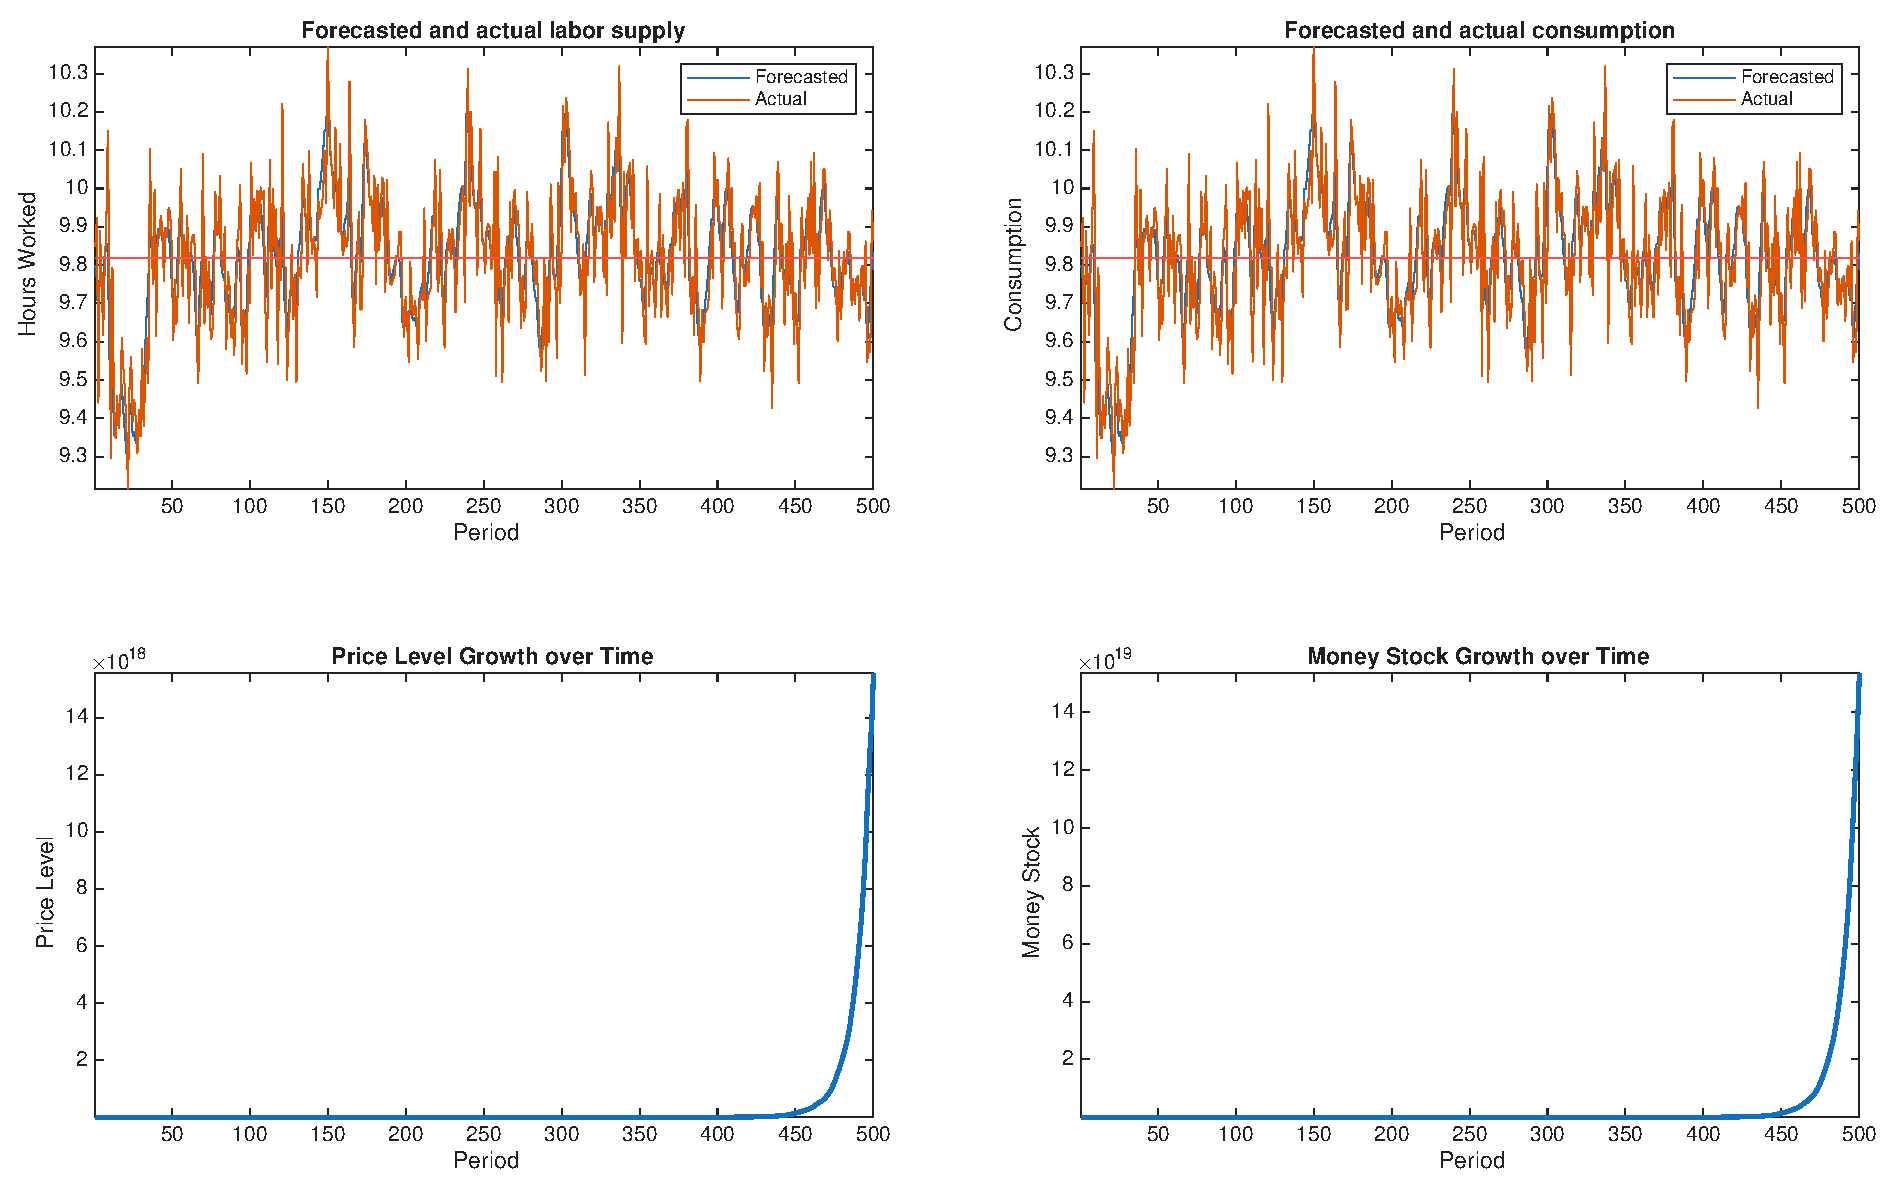
\includegraphics[width=0.7\textwidth]{figures/simulation.eps}%
    \vspace*{-0.15in}%
    \caption{Model simulations: 400 periods, $\rho=11$, $\beta=0.98$, $Z=1$, $B_\tau=0.01$, $\rho_\tau =0.5$, $\sigma_\tau=0.01$.}%
  \end{figure}%
\end{frame}%
%-------------------------------------------------------------------------
% Impulse Response Functions
\begin{frame}{Impulse Response Functions}%
  Impulse response functions (IRFs) are a nice way to \textbf{understand the dynamic implications of a model}. They are constructed as follows:%
  \begin{enumerate}%
    \item The prior value of the random variable is set equal to its mean:%
    \begin{align*}%
      \tau_{0} \; = \; \frac{B_{\tau}}{1-\rho_{\tau}}%
    \end{align*}%
    \pause%
    \item In period 1, $\varepsilon_{\tau,1} = 1$, so:%
    \begin{align*}%
      \tau_{1} \; = \; \frac{B_{\tau}}{1-\rho_{\tau}} + C%
    \end{align*}%
    \pause%
    \item After period 1 the shock is set to zero, so:%
    \begin{align*}%
      \tau_{t} \; = \; \frac{B_{\tau}}{1-\rho_{\tau}} + \rho_{\tau}^{t-1} C \quad \forall t \geq 1%
    \end{align*}%
    \pause%
    \item We then push these shocks through our model to trace what happens in period $t \geq 1$.%
    \pause%
    \item For each period we calculate the variables using the approach from slide \ref{slide:slove_model_steps}.%
  \end{enumerate}%
\end{frame}%
%-------------------------------------------------------------------------
% Impulse Response Functions of a Surprise Money Growth Shock
\begin{frame}{Impulse Response Functions of a Surprise Money Growth Shock}%
  \begin{figure}%
    \centering%
    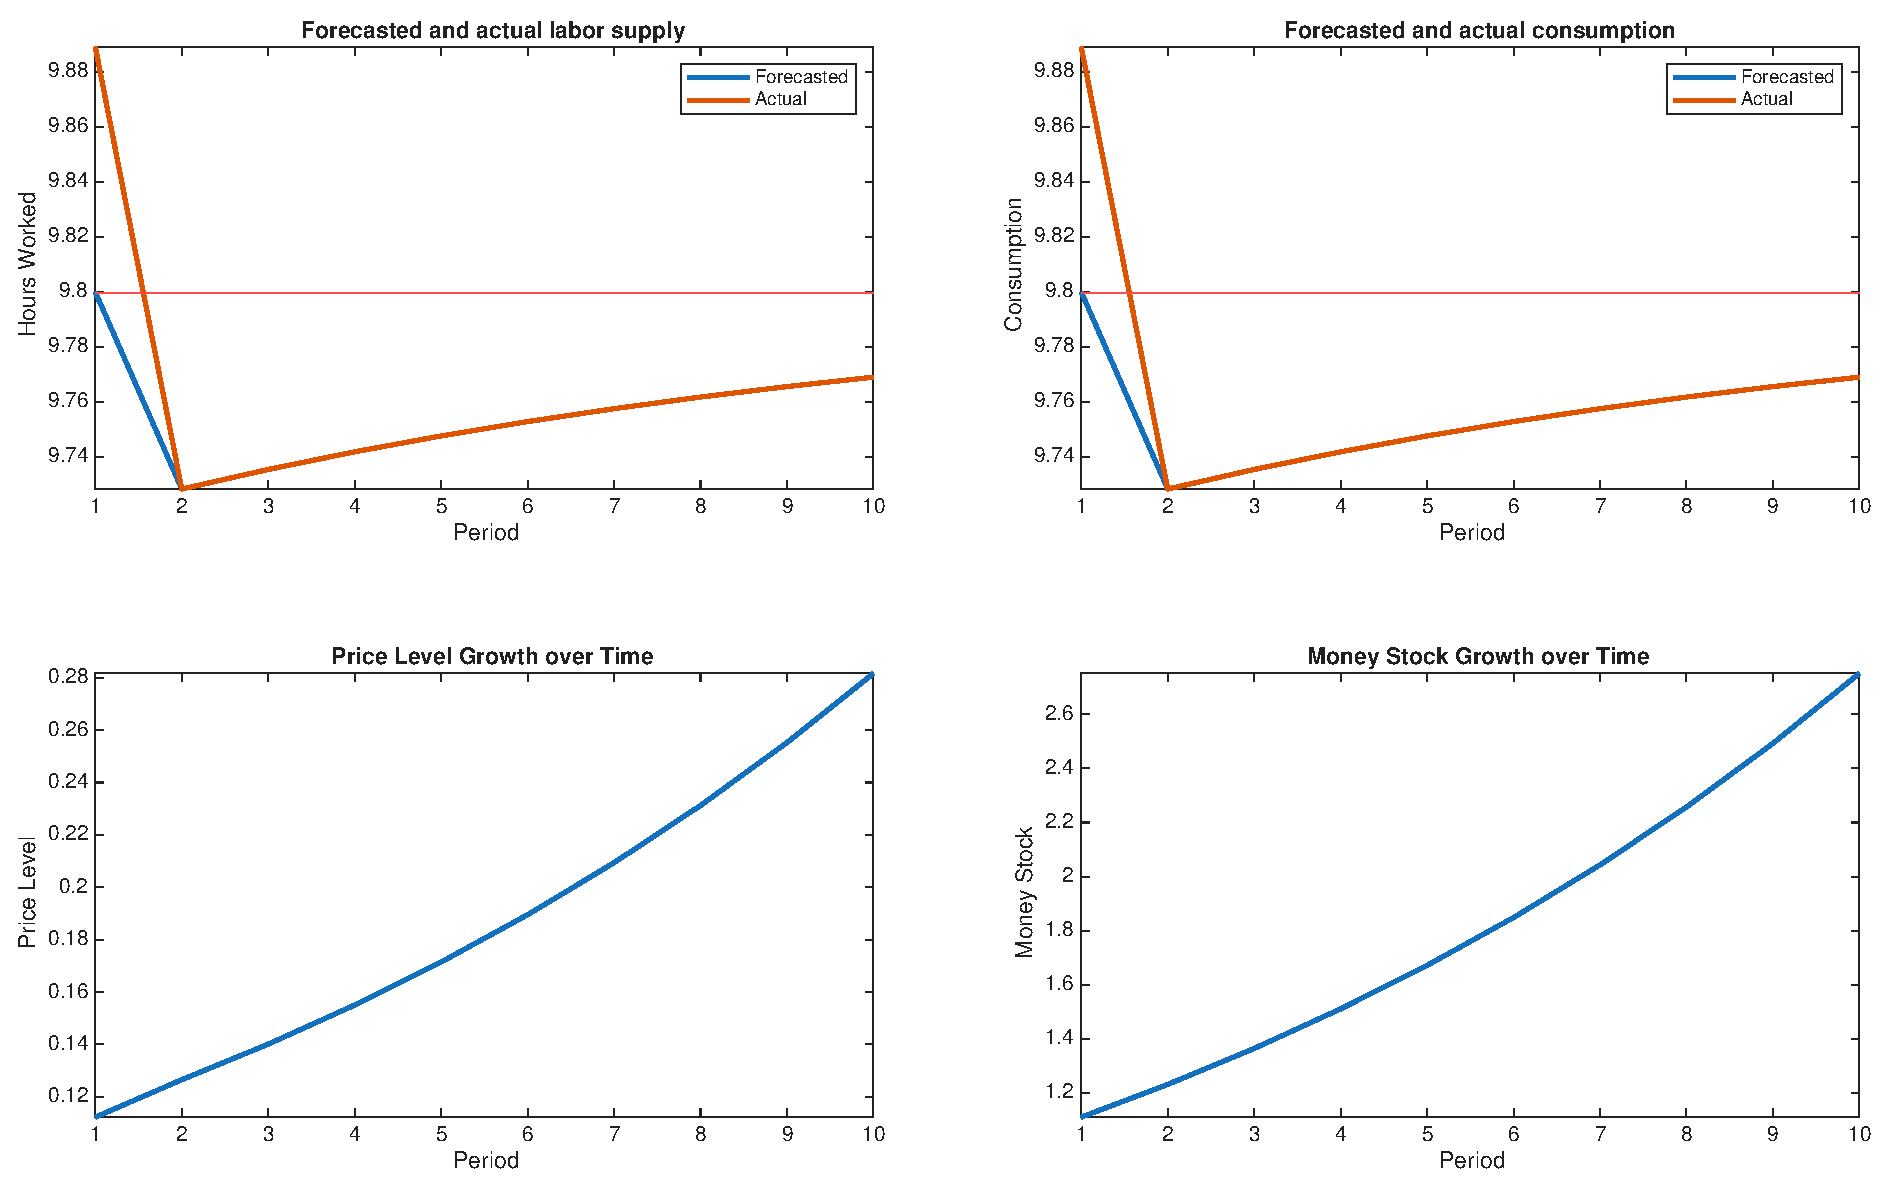
\includegraphics[width=0.7\textwidth]{figures/irf.eps}%
    \vspace*{-0.15in}%
    \caption{Impulse response functions: 40 periods (10 periods shown), $\rho=11$, $\beta=0.98$, $Z=1$, $B_\tau=0.01$, $\rho_\tau =0.5$, $\sigma_\tau=0.01$.}%
  \end{figure}%
\end{frame}%
%-------------------------------------------------------------------------
% CONCLUSIONS AND APPENDIX
%-------------------------------------------------------------------------
\section{Conclusion}%
%-------------------------------------------------------------------------
% Summarizing the Lecture
\begin{frame}{Summarizing the Lecture}%
  \begin{center}%
    \begin{large}%
      Can you summarize the three main aspects of the lecture?%
    \end{large}%
  \end{center}%
\end{frame}%
%-------------------------------------------------------------------------
% CONCLUSIONS
\begin{frame}{Concluding Remarks}%
  \begin{block}{Big Picture of the Lecture:}%
    \begin{enumerate}%
      \item How to set monetary policy goals, targets, and instruments?%
      \item How do households set their goods prices under market power?%
      \item What role does uncertain within period money growth play for aggregate demand?%
    \end{enumerate}%
  \end{block}%
  \pause%
  \begin{itemize}%
    \item[$\blacktriangleright$] \textbf{Monetary policy goals, targets, and instruments:}%
    \begin{itemize}%
      \item[$\rightarrow$] Implement observables targets with instruments of which we understand their economic channels well.%
    \end{itemize}%
    \item[$\blacktriangleright$] \textbf{Monopolistic competition and market power:}%
    \begin{itemize}%
      \item[$\rightarrow$] Each producer can set its own prices and has some market power to charge markups.%
      \item[$\rightarrow$] Yet, no aggregate demand effects of surprise money growth!% 
    \end{itemize}%
    \pause%
    \item[$\blacktriangleright$] \textbf{Information frictions and surprise inflation:}%
    \begin{itemize}%
      \item[$\rightarrow$] Surprise money growth can lead to an increase in aggregate demand.%
      \item[$\rightarrow$] Surprise money injections must come after prices are set and before households buy goods.%
    \end{itemize}%
    \pause%
    \item[$\blacktriangleright$] \textbf{Impulse response functions:}%
    \begin{itemize}%
      \item[$\rightarrow$] An important tool to disect and analyze the impact of a single shock on the model economy.%
    \end{itemize}%
  \end{itemize}%
\end{frame}%
%-------------------------------------------------------------------------
\begin{frame}{References}%
  \begin{itemize}%
    \item[$\blacktriangleright$] Harold L. Cole (2020). Monetary and Fiscal Policy through a DSGE Lens. Oxford University Press.%
    \item[$\blacktriangleright$] Taylor, J. B. (1993, December). Discretion versus policy rules in practice. In Carnegie-Rochester conference series on public policy (Vol. 39, pp. 195-214). North-Holland.%
  \end{itemize}%
\end{frame}%
%-------------------------------------------------------------------------
\end{document}%